\Opensolutionfile{ans}[ans/ans2D1-5-2]
\begin{vd}%[2D1Y5-1]%Ví dụ 1.
	\immini
	{Đường cong trong hình bên là đồ thị của một hàm số trong bốn hàm số được liệt kê ở bốn phương án A, B, C, D dưới đây. Hỏi hàm số đó là hàm số nào?
		\choice
		{$y=-x^3+3x^2-2$}
		{$y=x^3-3x-2$}
		{$y=-x^3+x^2-2$}
		{\True $y=-x^3+3x-2$}}
	{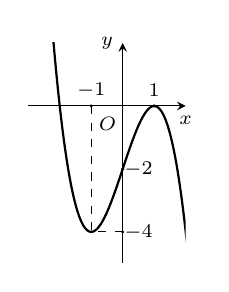
\begin{tikzpicture}[>=stealth,x=1cm,y=1cm,scale=0.4]
		\def\a{-1} 
		\def\b{0}
		\def\c{3}
		\def\d{-2}
		\draw[->] (-3,0) -- (2,0)node[below]{\scriptsize $x$};
		\draw[->] (0,-5) -- (0,2) node[left] {\scriptsize $y$};
		\draw (0,0)node[shift={(230:3mm)}]{\scriptsize $O$};
		\fill (-1,0)node[shift={(90:2mm)}]{\scriptsize $-1$}circle(1.5pt);
		\fill (1,0)node[shift={(90:2mm)}]{\scriptsize $1$}circle(1.5pt);
		\fill (0,-2)node[shift={(0:2mm)}]{\scriptsize $-2$}circle(1.5pt);
		\fill (0,-4)node[shift={(0:2mm)}]{\scriptsize $-4$}circle(1.5pt);
		\clip (-3,-5)rectangle(2,2);
		\draw[dashed] (-1,0)--(-1,-4)--(0,-4);
		\draw[thick,samples=150,smooth,domain=-5:5] plot(\x,{\a*(\x)^3+(\b)*(\x)^2+(\c)*\x+(\d)});
		\end{tikzpicture}}
	\loigiai{
		Dựa vào đồ thị ta thấy $a<0\Rightarrow$ Loại đáp án $y=x^3-3x-2$.\\
		ĐTHS đạt cực trị tại $x=\pm 1$ nên ta chọn đáp án $y=-x^3+3x-2$ vì có
		$y'=-3x^2+3=0\Leftrightarrow x=\pm 1$.}
\end{vd}
\begin{vd}%[2D1Y5-1]%Ví dụ 2.
	\immini
	{Đồ thị hình bên là đồ thị của một trong bốn đồ thị của hàm số ở các phương án A, B, C, D dưới đây. Hãy chọn phương án đúng
		\choice
		{$y=\dfrac{1}{4}x^4+2x^2+5$}
		{$y=-\dfrac{1}{4}x^4+2x^2+5$}
		{$y=-\dfrac{1}{4}x^4+5$}
		{\True $y=-\dfrac{1}{4}x^4-x^2+5$}}
	{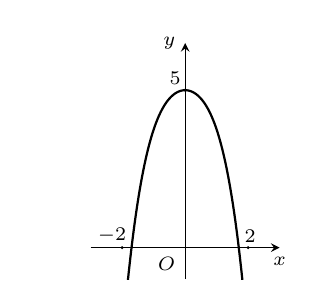
\begin{tikzpicture}[>=stealth,x=1cm,y=1cm,scale=0.4]
		\def\a{-1/4} 
		\def\b{-1}
		\def\c{5}
		\draw[->] (-3,0) -- (3,0) node[below] {\scriptsize $x$};
		\draw[->] (0,-1) -- (0,6.5) node[left] {\scriptsize $y$};
		\draw (0,0)node[below left]{\scriptsize $O$};
		\fill (-2,0)node[shift={(130:2mm)}]{\scriptsize $-2$}circle(1.5pt);
		\fill (2,0)node[shift={(80:1.5mm)}]{\scriptsize $2$}circle(1.5pt);
		\fill (0,5)node[shift={(130:2mm)}]{\scriptsize $5$}circle(1.5pt);
		\clip (-5,-1)rectangle(3,6.5);
		\draw[thick,samples=150,smooth,domain=-4:4] plot(\x,{\a*(\x)^4+(\b)*(\x)^2+(\c)});
		\end{tikzpicture}}
	\loigiai{
		Đồ thị có một cực đại suy ra $a.b\geq 0$ và $a\leq 0$, do đó loại hai phương án $y=\dfrac{1}{4}x^4+2x^2+5$ và $y=-\dfrac{1}{4}x^4+2x^2+5$.\\
		Đồ thị $y=-\dfrac{1}{4}x^4+5$ cắt $Ox$ tại hai điểm có hoành độ lần lượt là $x=\sqrt{\sqrt{20}}>2$ và $x=-\sqrt{\sqrt{20}} <-2$ nên loại $y=-\dfrac{1}{4}x^4+5$.}
\end{vd}
\begin{vd}%[2D1Y5-1]%Ví dụ 3.
	\immini
	{Đồ thị sau đây là của hàm số nào?
		\choice
		{\True $y=\dfrac{2x+1}{x+1}$}
		{$y=\dfrac{x+3}{1-x}$}
		{$y=\dfrac{x+2}{x+1}$}
		{$y=\dfrac{x-1}{x+1}$}}
	{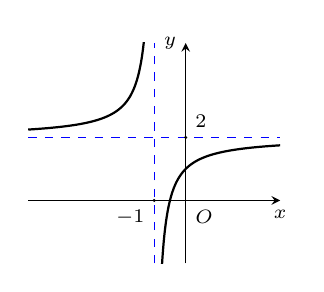
\begin{tikzpicture}[>=stealth,x=1cm,y=1cm,scale=0.4]
		\def\a{2}
		\def\b{1}
		\def\c{1}
		\def\d{1}
		\draw[->] (-5,0) -- (3,0) node[below] {\scriptsize $x$};
		\draw[->] (0,-2) -- (0,5) node[left] {\scriptsize $y$};
		\draw (0,0)node[below right]{\scriptsize $O$};
		\draw[dashed,blue] (-1,-2)--(-1,5) (-5,2)--(3,2);
		\fill (-1,0)node[below left]{\scriptsize $-1$}circle(1.5pt);
		\fill (0,2)node[above right]{\scriptsize $2$}circle(1.5pt);
		\clip (-5,-2)rectangle(3,5);
		\pgfmathsetmacro{\can}{-(\d)/(\c)}
		\draw[thick,samples=150,smooth,domain=-5:{\can-.1}] plot(\x,{(\a*\x+(\b))/(\c*\x+(\d))}); 
		\draw[thick,samples=150,smooth,domain={\can+.1}:5] plot(\x,{(\a*\x+(\b))/(\c*\x+(\d))}); 
		\end{tikzpicture}}
	\loigiai{
		Đồ thị hàm số nhận $x=-1$ là TCĐ và $y=2$ là TCN nên ta loại được đáp án $y=\dfrac{x+3}{1-x}$, $y=\dfrac{x+2}{x+1}$, $y=\dfrac{x-1}{x+1}$.}
\end{vd}
\begin{vd}%[2D1B5-2]%Ví dụ 4.
Hàm số $y=\dfrac{|2x-1|}{x+1}$ có đồ thị là hình vẽ nào trong bốn phương án A, B, C, D dưới đây?
\choice
{\True \begin{tikzpicture}[scale=0.5, font=\footnotesize, line join=round, line cap=round,>=stealth]
	\def\a{2} \def\b{-1} \def\c{1} \def\d{1} % Hệ số
	\def\xmin{-5} \def\xmax{4}
	\def\ymin{-2} \def\ymax{6}
	\draw[color=gray!50,dashed] (\xmin,\ymin) grid (\xmax,\ymax);
	\draw[->] (\xmin,0)--(\xmax,0) node [below]{$x$};
	\draw[->] (0,\ymin)--(0,\ymax) node [left]{$y$};
	\node at (0,0) [below left]{$O$};
	\clip (\xmin+0.1,\ymin+0.1) rectangle (\xmax-0.1,\ymax-0.1);
	\draw[smooth,samples=300,domain=\xmin:(-\d/\c-0.1)] plot(\x,{(\a*(\x)+\b)/(\c*(\x)+\d)});
	\draw[smooth,samples=300,domain=(-\d/\c+0.1:\xmax)] plot(\x,{(abs(\a*(\x)+\b))/(\c*(\x)+\d)});
	\draw[dashed] (-\d/\c,\ymin)--(-\d/\c,\ymax);
	\draw[dashed] (\xmin,\a/\c)--(\xmax,\a/\c);
	\fill (0,0) circle (1.0pt) (0.5,0) circle (1.0pt)node[below]{$\dfrac{1}{2}$};
	\end{tikzpicture}}
{\begin{tikzpicture}[scale=0.5, font=\footnotesize, line join=round, line cap=round,>=stealth]
	\def\a{2} \def\b{-1} \def\c{1} \def\d{1} % Hệ số
	\def\xmin{-5} \def\xmax{4}
	\def\ymin{-3.5} \def\ymax{6}
	\draw[color=gray!50,dashed] (\xmin,\ymin) grid (\xmax,\ymax);
	\draw[->] (\xmin,0)--(\xmax,0) node [below]{$x$};
	\draw[->] (0,\ymin)--(0,\ymax) node [left]{$y$};
	\node at (0,0) [below left]{$O$};
	\clip (\xmin+0.1,\ymin+0.1) rectangle (\xmax-0.1,\ymax-0.1);
	\draw[smooth,samples=300,domain=\xmin:(-\d/\c-0.1)] plot(\x,{(\a*(\x)+\b)/(\c*(\x)+\d)});
	\draw[smooth,samples=300,domain=(-\d/\c+0.1:\xmax)] plot(\x,{(-abs(\a*(\x)+\b))/(\c*(\x)+\d)});
	\draw[dashed] (-\d/\c,\ymin)--(-\d/\c,\ymax);
	\draw[dashed] (\xmin,\a/\c)--(\xmax,\a/\c);
	\fill (0,0) circle (1.0pt) (0.5,0) circle (1.0pt)node[above]{$\dfrac{1}{2}$};
	\end{tikzpicture}}
{\begin{tikzpicture}[scale=0.5, font=\footnotesize, line join=round, line cap=round,>=stealth]
	\def\a{2} \def\b{-1} \def\c{1} \def\d{1} % Hệ số
	\def\xmin{-5} \def\xmax{4}
	\def\ymin{-5.5} \def\ymax{4}
	\draw[color=gray!50,dashed] (\xmin,\ymin) grid (\xmax,\ymax);
	\draw[->] (\xmin,0)--(\xmax,0) node [below]{$x$};
	\draw[->] (0,\ymin)--(0,\ymax) node [left]{$y$};
	\node at (0,0) [below left]{$O$};
	\clip (\xmin+0.1,\ymin+0.1) rectangle (\xmax-0.1,\ymax-0.1);
	\draw[smooth,samples=300,domain=\xmin:(-\d/\c-0.1)] plot(\x,{(\a*(\x)+\b)/(abs(\c*(\x)+\d))});
	\draw[smooth,samples=300,domain=(-\d/\c+0.1:\xmax)] plot(\x,{(\a*(\x)+\b)/(\c*(\x)+\d)});
	\draw[dashed] (-\d/\c,\ymin)--(-\d/\c,\ymax);
	\draw[dashed] (\xmin,\a/\c)--(\xmax,\a/\c);
	\fill (0,0) circle (1.0pt) (0.5,0) circle (1.0pt)node[above]{$\dfrac{1}{2}$};
	\end{tikzpicture}}
{\begin{tikzpicture}[scale=0.5, font=\footnotesize, line join=round, line cap=round,>=stealth]
	\def\a{2} \def\b{-1} \def\c{1} \def\d{1} % Hệ số
	\def\xmin{-5} \def\xmax{4}
	\def\ymin{-2} \def\ymax{6}
	\draw[color=gray!50,dashed] (\xmin,\ymin) grid (\xmax,\ymax);
	\draw[->] (\xmin,0)--(\xmax,0) node [below]{$x$};
	\draw[->] (0,\ymin)--(0,\ymax) node [left]{$y$};
	\node at (0,0) [below left]{$O$};
	\clip (\xmin+0.1,\ymin+0.1) rectangle (\xmax-0.1,\ymax-0.1);
	\draw[smooth,samples=300,domain=\xmin:(-\d/\c-0.1)] plot(\x,{(\a*(\x)+\b)/(\c*(\x)+\d)});
	\draw[smooth,samples=300,domain=(-\d/\c+0.1:\xmax)] plot(\x,{(-(\a*(\x)+\b))/(\c*(\x)+\d)});
	\draw[dashed] (-\d/\c,\ymin)--(-\d/\c,\ymax);
	\draw[dashed] (\xmin,\a/\c)--(\xmax,\a/\c);
	\fill (0,0) circle (1.0pt) (0.5,0) circle (1.0pt)node[below]{$\dfrac{1}{2}$};
	\end{tikzpicture}}
\loigiai{
	Ta có: $\lim\limits_{x\to+\infty}\dfrac{|2x-1|}{x+1}=2$; $\lim\limits_{x\to-\infty}\dfrac{|2x-1|}{x+1}=-2$.\\
	Giao của đồ thị hàm số $y=\dfrac{|2x-1|}{x+1}$ với trục $Ox,Oy$ lần lượt là điểm $A\left(\dfrac{1}{2};0\right),B(0;1)$.}
\end{vd}
\begin{vd}%[2D1B5-2]%Ví dụ 1.
	Cho hàm số $f(x)$ liên tục trên đoạn $[-2;2]$ và có đồ thị là đường cong như hình vẽ bên. Tìm số nghiệm của phương trình $|f(x)|=1$ trên đoạn $[-2;2]$. 
\begin{center}
	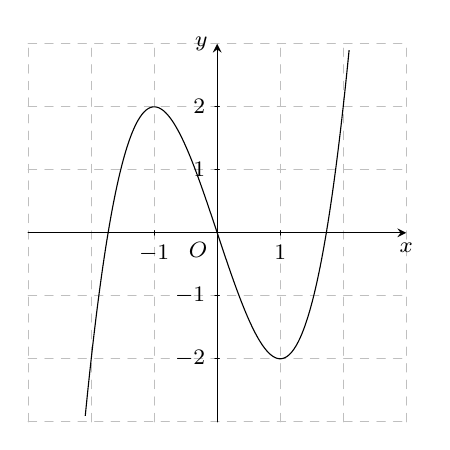
\begin{tikzpicture}[scale=0.8,>=stealth, font=\footnotesize, line join=round, line cap=round]
	\def\a{1} \def\b{0} \def\c{-3} \def\d{0} % Hệ số
	\def\xmin{-3} \def\xmax{3}
	\def\ymin{-3} \def\ymax{3} 
	\draw[color=gray!50,dashed] (\xmin,\ymin) grid (\xmax,\ymax); 
	\draw[->] (\xmin,0)--(\xmax,0) node [below]{$x$};
	\draw[->] (0,\ymin)--(0,\ymax) node [left]{$y$};
	\node at (0,0) [below left]{$O$};
	\foreach \x in {-1,1}
	\draw[thin] (\x,1pt)--(\x,-1pt) node [below] {$\x$};
	\foreach \y in {-2,-1,1,2}
	\draw[thin] (1pt,\y)--(-1pt,\y) node [left] {$\y$};
	\clip (\xmin+0.1,\ymin+0.1) rectangle (\xmax-0.5,\ymax-0.1);
	\draw[smooth,samples=300] plot(\x,{\a*(\x)^3+\b*(\x)^2+\c*(\x)+\d});
	\end{tikzpicture}
\end{center}
	\choice
	{$5$}
	{$3$}
	{$4$}
	{\True $6$}
	\loigiai{
		Số nghiệm của phương trình $|f(x)|=1$ bằng số giao điểm của đồ thị hàm số $y=1$ và $y=|f(x)|$.\\
		Đồ thị của hàm số $y=|f(x)|$ được suy ra từ đồ thị hàm số $f(x)$ như hình vẽ.
		\begin{center}
			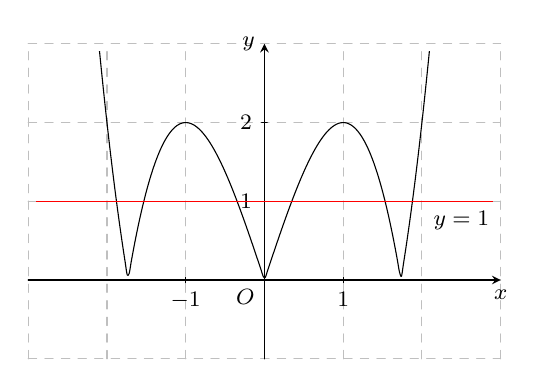
\begin{tikzpicture}[scale=1,>=stealth, font=\footnotesize, line join=round, line cap=round]
			\def\a{1} \def\b{0} \def\c{-3} \def\d{0} % Hệ số
			\def\xmin{-3} \def\xmax{3}
			\def\ymin{-1} \def\ymax{3} 
			\draw[color=gray!50,dashed] (\xmin,\ymin) grid (\xmax,\ymax); 
			\draw[->] (\xmin,0)--(\xmax,0) node [below]{$x$};
			\draw[->] (0,\ymin)--(0,\ymax) node [left]{$y$};
			\node at (0,0) [below left]{$O$};
			\foreach \x in {-1,1}
			\draw[thin] (\x,1pt)--(\x,-1pt) node [below] {$\x$};
			\foreach \y in {1,2}
			\draw[thin] (1pt,\y)--(-1pt,\y) node [left] {$\y$};
			\clip (\xmin+0.1,\ymin+0.1) rectangle (\xmax-0.1,\ymax-0.1);
			\draw[smooth,samples=400] plot(\x,{abs(\a*(\x)^3+\b*(\x)^2+\c*(\x)+\d)});
			\draw[red] (-2.9,1)--(2.9,1);
			\node at (2.5,1) [below]{$y=1$};
			\end{tikzpicture}
		\end{center}
			Dựa vào đồ thị ta thấy phương trình $|f(x)|=1$ luôn có 6 nghiệm.}
\end{vd}
\begin{vd}%[2D1K5-2]%Ví dụ 2.
	Cho hàm số $y=f(x)$ có bảng biến thiên như sau: 
	\begin{center}
		
\begin{tikzpicture}
		\tkzTabInit[nocadre=false,lgt=1.2,espcl=2.5,deltacl=0.6]
		{$x$ /0.6, $f'(x)$ /0.6, $f(x)$ /2.5}
		{$-\infty$,$0$,$2$,$+\infty$}
		\tkzTabLine{,-,$0$,+,$0$,-,}
		\tkzTabVar{+/$+\infty$,-/$-2$,+/$2$,-/$-\infty$}
		\end{tikzpicture}
	\end{center}
	Hỏi đồ thị hàm số $y=\left|f(x)+2\right|$ có tất cả bao nhiêu điểm cực trị?
	\choice
	{$2$}
	{$5$}
	{\True $3$}
	{$4$}
	\loigiai{
		Đặt $g(x)=f(x)+2$. Ta có $g'(x)=f'(x)$.\\
		Bảng biến thiên: \\
		\begin{center}
			
\begin{tikzpicture}
			\tkzTabInit[nocadre=false,lgt=1.2,espcl=2.5,deltacl=0.6]
			{$x$ /0.6, $g'(x)$ /0.6, $g(x)$ /2.5}
			{$-\infty$,$0$,$2$,$+\infty$}
			\tkzTabLine{,-,$0$,+,$0$,-,}
			\tkzTabVar{+/$+\infty$,-/$0$,+/$4$,-/$-\infty$}
			\end{tikzpicture}
		\end{center}
		Vậy đồ thị hàm số $y=\left|g(x)\right|$ có dạng: 
		\begin{center}
			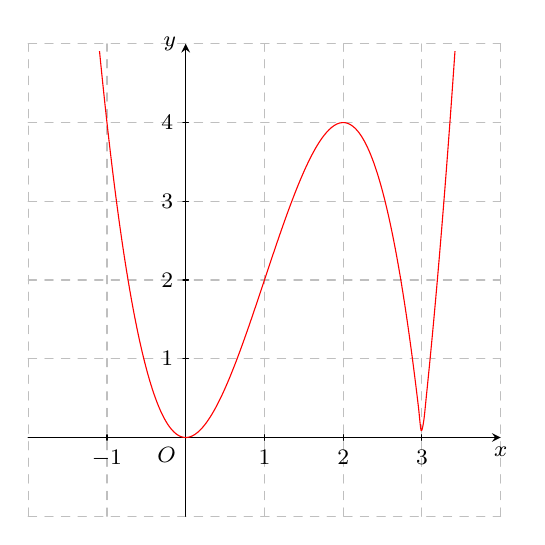
\begin{tikzpicture}[scale=1,>=stealth, font=\footnotesize, line join=round, line cap=round]
		\def\a{-1} \def\b{3} \def\c{0} \def\d{0} % Hệ số
		\def\xmin{-2} \def\xmax{4}
		\def\ymin{-1} \def\ymax{5} 
		\draw[color=gray!50,dashed] (\xmin,\ymin) grid (\xmax,\ymax);
		\draw[->] (\xmin,0)--(\xmax,0) node [below]{$x$};
		\draw[->] (0,\ymin)--(0,\ymax) node [left]{$y$};
		\node at (0,0) [below left]{$O$};
		\foreach \x in {-1,1,2,3}
		\draw[thin] (\x,1pt)--(\x,-1pt) node [below] {$\x$};
		\foreach \y in {1,2,3,4}
		\draw[thin] (1pt,\y)--(-1pt,\y) node [left] {$\y$};
		\clip (\xmin+0.1,\ymin+0.1) rectangle (\xmax-0.1,\ymax-0.1);
		\draw[smooth,samples=300,red] plot(\x,{abs(\a*(\x)^3+\b*(\x)^2+\c*(\x)+\d)});
		\end{tikzpicture}
		\end{center}		
		Do đó đồ thị hàm số $y=\left|f(x)+2\right|$ có tất cả $3$ điểm cực trị.}
\end{vd}
\begin{vd}%[2D1K5-2]%Ví dụ 3.
	Bảng biến thiên sau là của hàm số nào dưới đây?
	\begin{center}
			
\begin{tikzpicture}
			\tkzTabInit[nocadre=false,lgt=1.2,espcl=2.5,deltacl=0.6]
			{$x$ /0.6,$y'$ /0.6,$y$ /2}
			{$-\infty$,$-1$,$0$,$1$,$+\infty$}
			\tkzTabLine{,-,$0$,+,$0$,-,$0$,+,}
			\tkzTabVar{+/$+\infty$, -/$-4$,+/$-3$,-/$-4$,+/$+\infty$}
			\end{tikzpicture}
	\end{center}
	\choice
	{$y=\dfrac{1}{2}x^4-x^2-3$}
	{$y=2x^4-4x^2-3$}
	{$y=2|x|^3-3|x|-3$}
	{\True $y=2|x^3|-3x^2-3$}
	\loigiai{
		Loại hai đáp án A và B vì đồ thị hàm số không chứa điểm cực trị $M(1;-4)$.\\
		Loại đáp án C vì:\\
		Với $x\geq 0$, ta có $y=2|x|^3-3|x|-3=2x^3-3x-3$, nên $y'=6x^2-3$.\\
		$y'=0\Leftrightarrow 6x^2-3=0\Leftrightarrow\hoac{&x=\dfrac{1}{\sqrt{2}}\\&x=\dfrac{-1}{\sqrt{2}}<0(l)}\Rightarrow x=\dfrac{1}{\sqrt{2}}$ là hoành độ điểm cực trị của đồ thị hàm số.\\
		Vậy đáp án chọn là đáp án $D$.}
\end{vd}
\begin{vd}%[2D1K5-2]%Ví dụ 4.
	Cho hàm số $f(x)=\left|x^3-3x^2+m\right|$ với $m\in[-5;5]$ là tham số. Có bao nhiêu giá trị nguyên của $m$ để hàm số $f(x)$ có đúng ba điểm cực trị. 
	\choice
	{$3$}
	{$0$}
	{\True $8$}
	{$6$}
	\loigiai{
		Xét hàm số $g(x)=x^3-3x^2+m$ có $g'(x)=0\Leftrightarrow 3x^2-6x=0\Leftrightarrow\hoac{&x=0\\&x=2.}$ \\
		Bảng biến thiên
		\begin{center}
			
\begin{tikzpicture}
			\tkzTabInit[nocadre=false,lgt=1.2,espcl=2.5,deltacl=0.6]
			{$x$ /0.6, $g'(x)$ /0.6, $g(x)$ /2.5}
			{$-\infty$,$0$,$2$,$+\infty$}
			\tkzTabLine{,+,$0$,-,$0$,+,}
			\tkzTabVar{-/$-\infty$,+/$m$,-/$-4+m$,+/$+\infty$}
			\end{tikzpicture}
		\end{center}
		Từ bảng biến thiên ta thấy để hàm số $f(x)$ có đúng ba điểm cực trị thì đồ thị hàm số $g(x)$ phải có đúng một giao điểm hoặc tiếp xúc với $Ox$.\\
		Điều kiện này tương đương với $\hoac{&m\leq 0\\&-4+m\geq 0}\Leftrightarrow\hoac{&m\leq 0\\&m\geq 4.}$ \\
		Kết hợp điều kiện $m\in[-5;5]$ ta có $m\in\left\{-5;-4;-3;-2;-1;0;4;5\right\}$. Vậy có 8 giá trị thoả mãn.}
\end{vd}
\begin{vd}%[2D1K5-2]%Ví dụ 5.
	Cho hàm số $f(x)=x^3-3x^2+x+\dfrac{3}{2}$. Phương trình $\dfrac{f\left(f(x)\right)}{2f(x)-1}=1$ có bao nhiêu nghiệm thực phân biệt?
	\choice
	{$4$ nghiệm}
	{$9$ nghiệm}
	{$6$ nghiệm}
	{\True $5$ nghiệm}
	\loigiai{
		Điều kiện: $f(x)\neq\dfrac{1}{2}\Leftrightarrow x^3-3x^2+x+1\neq 0\Leftrightarrow\heva{&x\neq 1\\&x\neq 1\pm\sqrt{2}.}$ \\
		Xét hàm số $y=f(x)$ có $f'(x)=3x^2-6x+1$; $f'(x)=0\Leftrightarrow x=\dfrac{3\pm\sqrt{6}}{3}$.\\
		Chia $f(x)$ cho $f'(x)$ ta được: $f(x)=p(x)\cdot f'(x)+\dfrac{11}{6}-\dfrac{4}{3}x$.\\
		$f\left(\dfrac{3+\sqrt{6}}{3}\right)=\dfrac{1}{2}-\dfrac{4\sqrt{6}}{9}\approx-0,59$; $f\left(\dfrac{3-\sqrt{6}}{3}\right)=\dfrac{1}{2}+\dfrac{4\sqrt{6}}{9}\approx 1,59$.\\
		Bảng biến thiên: 
		\begin{center}
			\begin{tikzpicture}
			\tkzTabInit[nocadre=false,lgt=1.2,espcl=2.5,deltacl=0.6]
			{$x$ /0.6, $y'$ /0.6, $y$ /2.5}
			{$-\infty$,$\frac{3-\sqrt{6}}{3}$,$\frac{3+\sqrt{6}}{3}$ ,$+\infty$}
			\tkzTabLine{,+,$0$,-,$0$,+,}
			\tkzTabVar{-/$-\infty$,+/$y_{\text{CĐ}}$,-/$y_{\text{CT}}$,+/$+\infty$}
			\end{tikzpicture}
		\end{center}
		Đặt $t=f(x),t\neq\dfrac{1}{2}$.\\
		Phương trình $\dfrac{f\left(f(x)\right)}{2f(x)-1}=1\Leftrightarrow f(t)=2t-1$ \\
		$ \Leftrightarrow t^3-3t^2+t+\dfrac{3}{2}=2t-1\Leftrightarrow g(t)=t^3-3t^2-t+\dfrac{5}{2}=0\Leftrightarrow\hoac{&t=t_1\approx 3,06\\&t=t_2\approx 0,87\\&t=t_3\approx-0,93} $ (thỏa mãn).\\
		(Ở đây dùng máy tính để tìm nghiệm xấp xỉ, hoặc có thể sử dụng kiến thức lớp 11 để chứng minh phương trình có 3 nghiệm phân biệt: $t_1\in(3;4), t_2\in(0;1), t_3\in\left(-1;-\dfrac{3}{5}\right)$).\\
		Với $t=t_1\Leftrightarrow f(x)=t_1\approx 3,06$, từ đồ thị ta thấy phương trình này chỉ cho 1 nghiệm.\\
		Với $t=t_2\Leftrightarrow f(x)=t_2\approx 0,87$, từ đồ thị ta thấy phương trình này cho 3 nghiệm.\\
		Với $t=t_3\Leftrightarrow f(x)=t_3\approx-0,93 <-0,59$, từ đồ thị ta thấy phương trình này chỉ cho 1 nghiệm.\\
		Vậy phương trình đã cho có 5 nghiệm phân biệt.}
\end{vd}
\paragraph{Câu hỏi trắc nghiệm}
\begin{ex}%[2D1Y5-1]%Câu 1.
\immini
{Đường cong như hình vẽ là đồ thị của một trong các hàm số dưới đây. Hàm số đó là hàm số nào?
	\choice
	{$y=(x-1)(x-2)^2$}
	{$y=(x+1)(x+2)^2$}
	{$y=(x-1)(x+2)^2$}
	{\True $y=(x-1)^2(x+2)$}}
{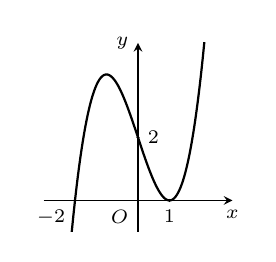
\begin{tikzpicture}[>=stealth,x=1cm,y=1cm,scale=0.4]
	\def\a{1} 
	\def\b{0}
	\def\c{-3}
	\def\d{2}
	\draw[->] (-3,0) -- (3,0)node[below]{\scriptsize $x$};
	\draw[->] (0,-1) -- (0,5) node[left] {\scriptsize $y$};
	\draw (0,0)node[below left]{\scriptsize $O$};
	\fill (-2,0)node[below left]{\scriptsize $-2$}circle(1.5pt);
	\fill (1,0)node[below]{\scriptsize $1$}circle(1.5pt);
	\fill (0,2)node[right]{\scriptsize $2$}circle(1.5pt);
	\clip (-3,-1)rectangle(3,5);
	\draw[thick,samples=150,smooth,domain=-3:3] plot(\x,{\a*(\x)^3+(\b)*(\x)^2+(\c)*\x+(\d)});
	\end{tikzpicture}}
\loigiai{
	Do đồ thị hàm số cắt trục $Ox$ tại điểm $(-2;0)$ và tiếp xúc với $Ox$ tại điểm $(1;0)$ nên hàm số $y=(x-1)^2(x+2)$ thỏa mãn.}
\end{ex}
\begin{ex}%[2D1Y5-1]%Câu 2.
\immini
{Đường cong hình bên dưới là đồ thị của một hàm số trong bốn hàm số được liệt kê ở bốn phương án A, B, C, D dưới đây. Hỏi hàm số đó là hàm số nào?
	\choice
	{$y=x^3+3x^2+2$}
	{$y=-x^3-3x^2+2$}
	{$y=\dfrac{2x+1}{x-1}$}
	{\True $y=x^3-3x^2+2$}}
{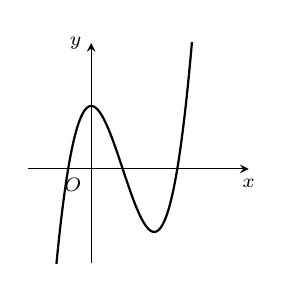
\begin{tikzpicture}[>=stealth,x=1cm,y=1cm,scale=0.4]
	\def\a{1}
	\def\b{-3}
	\def\c{0}
	\def\d{2}
	\draw[->] (-2,0) -- (5,0)node[below]{\scriptsize $x$};
	\draw[->] (0,-3) -- (0,4) node[left] {\scriptsize $y$};
	\draw (0,0)node[below left]{\scriptsize $O$};
	\clip (-2,-3)rectangle(5,4);
	\draw[thick,samples=150,smooth,domain=-2:5] plot(\x,{\a*(\x)^3+(\b)*(\x)^2+(\c)*\x+(\d)});
	\end{tikzpicture}
}
\loigiai{
	Đồ thị hàm số là đồ thị hàm bậc ba với $a>0$ nên loại hàm số $y=-x^3-3x^2+2$ và $y=\dfrac{2x+1}{x-1}$.\\
	Hàm số có $2$ điểm cực trị $x=0$ và $x=x_2>0$ nên loại $y=x^3+3x^2+2$.}
\end{ex}
\begin{ex}%[2D1Y5-1]%Câu 3.
Đồ thị của hàm số $y=x^3-3x^2+4x-1$ là hình nào dưới đây?
\choice
{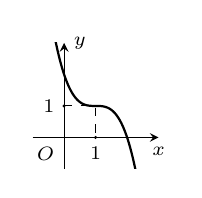
\begin{tikzpicture}[>=stealth,x=1cm,y=1cm,scale=0.4]
	\def\a{-1} 
	\def\b{3}
	\def\c{-3}
	\def\d{2}
	\draw[->] (-1,0) -- (3,0)node[below]{\scriptsize $x$};
	\draw[->] (0,-1) -- (0,3) node[right] {\scriptsize $y$};
	\draw (0,0)node[below left]{\scriptsize $O$};
	\fill (1,0)node[below]{\scriptsize $1$}circle(1.5pt);
	\fill (0,1)node[left]{\scriptsize $1$}circle(1.5pt);
	\draw[dashed] (0,1)--(1,1)--(1,0);
	\clip (-1,-1)rectangle(3,3);
	\draw[thick,samples=150,smooth,domain=-1:3] plot(\x,{\a*(\x)^3+(\b)*(\x)^2+(\c)*\x+(\d)});
	\end{tikzpicture}
}
{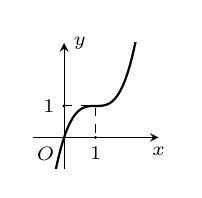
\begin{tikzpicture}[>=stealth,x=1cm,y=1cm,scale=0.4]
	\def\a{1} 
	\def\b{-3}
	\def\c{3}
	\def\d{0}
	\draw[->] (-1,0) -- (3,0)node[below]{\scriptsize $x$};
	\draw[->] (0,-1) -- (0,3) node[right] {\scriptsize $y$};
	\draw (0,0)node[below left]{\scriptsize $O$};
	\fill (1,0)node[below]{\scriptsize $1$}circle(1.5pt);
	\fill (0,1)node[left]{\scriptsize $1$}circle(1.5pt);
	\draw[dashed] (0,1)--(1,1)--(1,0);
	\clip (-1,-1)rectangle(3,3);
	\draw[thick,samples=150,smooth,domain=-1:3] plot(\x,{\a*(\x)^3+(\b)*(\x)^2+(\c)*\x+(\d)});
	\end{tikzpicture}
}
{\True 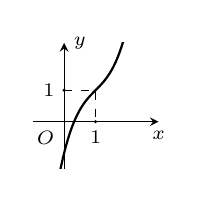
\begin{tikzpicture}[>=stealth,x=1cm,y=1cm,scale=0.4]
	\def\a{1} 
	\def\b{-3}
	\def\c{4}
	\def\d{-1}
	\draw[->] (-1,0) -- (3,0)node[below]{\scriptsize $x$};
	\draw[->] (0,-1.5) -- (0,2.5) node[right] {\scriptsize $y$};
	\draw (0,0)node[below left]{\scriptsize $O$};
	\fill (1,0)node[below]{\scriptsize $1$}circle(1.5pt);
	\fill (0,1)node[left]{\scriptsize $1$}circle(1.5pt);
	\draw[dashed] (0,1)--(1,1)--(1,0);
	\clip (-1,-1.5)rectangle(3,2.5);
	\draw[thick,samples=150,smooth,domain=-1:3] plot(\x,{\a*(\x)^3+(\b)*(\x)^2+(\c)*\x+(\d)});
	\end{tikzpicture}
}
{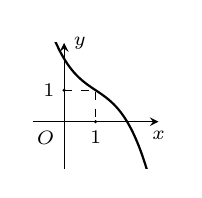
\begin{tikzpicture}[>=stealth,x=1cm,y=1cm,scale=0.4]
	\def\a{-1/3} 
	\def\b{1}
	\def\c{-5/3}
	\def\d{2}
	\draw[->] (-1,0) -- (3,0)node[below]{\scriptsize $x$};
	\draw[->] (0,-1.5) -- (0,2.5) node[right] {\scriptsize $y$};
	\draw (0,0)node[below left]{\scriptsize $O$};
	\fill (1,0)node[below]{\scriptsize $1$}circle(1.5pt);
	\fill (0,1)node[left]{\scriptsize $1$}circle(1.5pt);
	\draw[dashed] (0,1)--(1,1)--(1,0);
	\clip (-1,-1.5)rectangle(3,2.5);
	\draw[thick,samples=150,smooth,domain=-1:3] plot(\x,{\a*(\x)^3+(\b)*(\x)^2+(\c)*\x+(\d)});
	\end{tikzpicture}
}
\loigiai{
	Đồ thị của hàm số $y=x^3-3x^2+4x-1$ cắt trục tại điểm có tung độ bằng $-1$.}
\end{ex}
\begin{ex}%[2D1Y5-1]%Câu 4.
\immini
{Đây là đồ thị của hàm số nào?
	\choice
	{$y=-x^3+3x^2+2$}
	{\True $y=x^3-3x^2+2$}
	{$y=-x^3+3x^2-2$}
	{$y=x^3-3x^2-2$}}
{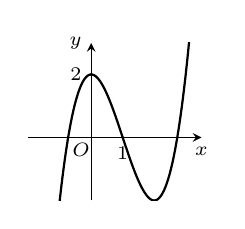
\begin{tikzpicture}[>=stealth,x=1cm,y=1cm,scale=0.4]
	\def\a{1} 
	\def\b{-3}
	\def\c{0}
	\def\d{2}
	\draw[->] (-2,0) -- (3.5,0)node[below]{\scriptsize $x$};
	\draw[->] (0,-2) -- (0,3) node[left] {\scriptsize $y$};
	\draw (0,0)node[shift={(230:2mm)}]{\scriptsize $O$};
	\fill (1,0)node[below]{\scriptsize $1$}circle(1.5pt);
	\fill (0,2)node[left]{\scriptsize $2$}circle(1.5pt);
	\clip (-2,-2)rectangle(3.5,3);
	\draw[thick,samples=150,smooth,domain=-2:3.5] plot(\x,{\a*(\x)^3+(\b)*(\x)^2+(\c)*\x+(\d)});
	\end{tikzpicture}
}
\loigiai{
	Từ đồ thị suy ra hệ số $a>0$ nên loại hàm số $y=-x^3+3x^2+2$ và $y=-x^3+3x^2-2$.\\
	Đồ thị cắt trục tung tại điểm có tung độ bằng $2$ nên loại hàm số $y=x^3-3x^2-2$.}
\end{ex}
\begin{ex}%[2D1Y5-1]%Câu 5.
\immini
{Đường cong trong hình bên là đồ thị của một trong bốn hàm số nào sau đây?
	\choice
	{\True $y=-x^4+2x^2$}
	{$y=x^4-2x^2$}
	{$y=-x^2+2x$}
	{$y=x^3+2x^2-x-1$}}
{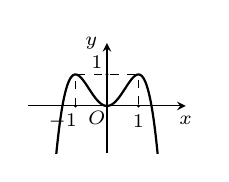
\begin{tikzpicture}[>=stealth,x=1cm,y=1cm,scale=0.4]
	\def\a{-1} 
	\def\b{2}
	\def\c{0}
	\draw[->] (-2.5,0) -- (2.5,0) node[below] {\scriptsize $x$};
	\draw[->] (0,-1.5) -- (0,2) node[left] {\scriptsize $y$};
	\draw (0,0)node[shift={(230:2mm)}]{\scriptsize $O$};
	\fill (-1,0)node[shift={(230:2.5mm)}]{\scriptsize $-1$}circle(1.5pt);
	\fill (1,0)node[shift={(270:2mm)}]{\scriptsize $1$}circle(1.5pt);
	\fill (0,1)node[shift={(130:2mm)}]{\scriptsize $1$}circle(1.5pt);
	\draw[dashed] (-1,0)--(-1,1)--(1,1)--(1,0);
	\clip (-2.5,-1.5)rectangle(2.5,2);
	\draw[thick,samples=150,smooth,domain=-2.5:2.5] plot(\x,{\a*(\x)^4+(\b)*(\x)^2+(\c)});
	\end{tikzpicture}} 
\loigiai{
	Đây là đồ thị hàm số bậc bốn trùng phương và có hệ số $a<0$.}
\end{ex}
\begin{ex}%[2D1Y5-1]%Câu 6.
\immini 
{Đường cong trong hình bên dưới là đồ thị của một hàm số trong bốn hàm số được liệt kê ở bốn phương án $A, B, C, D$ dưới đây. Hỏi hàm số đó là hàm số nào?
	\choice
	{$y=-x^3+3x+2$}
	{$y=x^3-3x$}
	{\True $y=-x^3+3x$}
	{$y=x^4-x^2+2$}}
{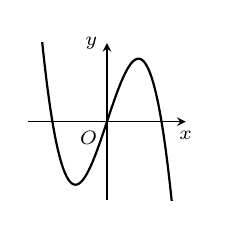
\begin{tikzpicture}[>=stealth,x=1cm,y=1cm,scale=0.4]
	\def\a{-1} 
	\def\b{0}
	\def\c{3}
	\def\d{0}
	\draw[->] (-2.5,0) -- (2.5,0)node[below]{\scriptsize $x$};
	\draw[->] (0,-2.5) -- (0,2.5) node[left] {\scriptsize $y$};
	\draw (0,0)node[below left]{\scriptsize $O$};
	\clip (-2.5,-2.5)rectangle(2.5,2.5);
	\draw[thick,samples=150,smooth,domain=-2.5:2.5] plot(\x,{\a*(\x)^3+(\b)*(\x)^2+(\c)*\x+(\d)});
	\end{tikzpicture}
}
\loigiai{
	Dựa vào đồ thị ta thấy, đồ thị đã cho là đồ thị hàm số bậc ba, đi qua gốc tọa độ và có hệ số $a<0$.}
\end{ex}
\begin{ex}%[2D1Y5-1]%Câu 7.
Bảng biến thiên sau đây là của hàm số
\begin{center}
	
\begin{tikzpicture}[>=stealth]
	\tkzTabInit[nocadre=false,lgt=1,espcl=2,deltacl=0.5]{$x$/.7 ,$y'$/.7,$y$/2}
	{$-\infty$ , $-1$ , $+\infty$}
	\tkzTabLine{ , - , d , - , }
	\tkzTabVar{+/$2$ , -D+/$-\infty$/$+\infty$ , -/$2$}
	\end{tikzpicture}
\end{center}
\choice
{$y=\dfrac{2x-1}{x-1}$}
{$y=\dfrac{2x-2}{x+1}$}
{\True $y=\dfrac{2x+3}{x+1}$}
{$y=\dfrac{x+2}{2x+2}$}
\loigiai{
	Từ BBT, đồ thị hàm số có đường tiệm cận đứng $x=-1$, đường tiệm cận ngang $y=2$ nên loại hàm số $y=\dfrac{2x-1}{x-1}$ và $y=\dfrac{x+2}{2x+2}$.\\
	Từ BBT, $y'<0,\forall x\in(-\infty;-1)\cup(-1;+\infty)$ nên loại hàm số $y=\dfrac{2x-2}{x+1}$.}
\end{ex}
\begin{ex}%[2D1Y5-1]%Câu 8.
Bảng biến thiên sau đây là của hàm số nào?
\begin{center}
	
\begin{tikzpicture}[>=stealth]
	\tkzTabInit[nocadre=false,lgt=1,espcl=2,deltacl=0.5]{$x$/.7 ,$y'$/.7,$y$/2}
	{$-\infty$ , $1$ , $+\infty$}
	\tkzTabLine{ , + , $0$ , + , }
	\tkzTabVar{-/$-\infty$ , R , +/$+\infty$}
	\tkzTabIma{1}{3}{2}{$1$}
	\end{tikzpicture}
\end{center}
\choice
{$y=-x^3+3x^2-3x$}
{$y=-x^3-3x^2-3x$}
{$y=x^3+3x^2-3x$}
{\True $y=x^3-3x^2+3x$}
\loigiai{
	$y=x^3-3x^2+3x\Rightarrow y'=3x^2-6x+3\Rightarrow y'=0\Leftrightarrow x=1$.}
\end{ex}
\begin{ex}%[2D1Y5-1]%Câu 9.
\immini 
{Hình vẽ sau đây là hình dạng đồ thị của hàm số nào
	\choice
	{$y=\dfrac{x+2}{x+1}$}
	{\True $y=\dfrac{x+2}{x-1}$}
	{$y=\dfrac{x-2}{x-1}$}
	{$y=\dfrac{x}{x-1}$}}
{\begin{tikzpicture}[>=stealth,x=1cm,y=1cm,scale=0.4]
	\def\a{1}
	\def\b{2}
	\def\c{1}
	\def\d{-1}
	\draw[->] (-4,0) -- (6,0) node[below] {\scriptsize $x$};
	\draw[->] (0,-4) -- (0,6) node[left] {\scriptsize $y$};
	\draw (0,0)node[below left]{\scriptsize $O$};
	\fill (1,0)node[below right]{\scriptsize $1$}circle(1.5pt);
	\fill (0,1)node[above left]{\scriptsize $1$}circle(1.5pt);
	\draw[dashed,blue] (1,-4)--(1,6) (-4,1)--(6,1);
	\clip (-4,-4)rectangle(6,6);
	\pgfmathsetmacro{\can}{-(\d)/(\c)}
	\draw[thick,samples=150,smooth,domain=-4:{\can-.1}] plot(\x,{(\a*\x+(\b))/(\c*\x+(\d))});
	\draw[thick,samples=150,smooth,domain={\can+.1}:6] plot(\x,{(\a*\x+(\b))/(\c*\x+(\d))});
	\end{tikzpicture}}
\loigiai{
	Dựa vào đồ thị ta thấy hàm số luôn nghịch biến trên từng khoảng xác định và có phương trình hai đường tiệm cận là $x=1$ và $y=1$ và cắt trục tung tại điểm có tọa độ $(0;-2)$ nên hàm số phải là $y=\dfrac{x+2}{x-1}$.}
\end{ex}
\begin{ex}%[2D1Y5-1]%Câu 10.
\immini 
{Đường cong trong hình bên là đồ thị của một hàm số trong bốn hàm số dưới đây. Hỏi hàm số đó là hàm số nào?
	\choice
	{$y=\dfrac{2x+1}{2x-2}$}
	{$y=\dfrac{-x}{1-x}$}
	{$y=\dfrac{x-1}{x+1}$}
	{\True $y=\dfrac{x+1}{x-1}$}}
{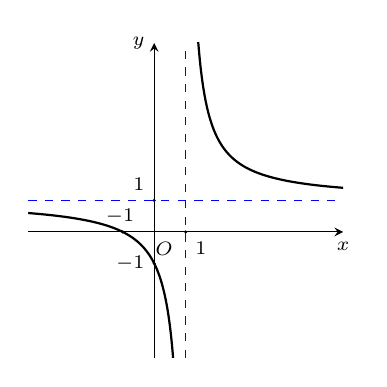
\begin{tikzpicture}[>=stealth,x=1cm,y=1cm,scale=0.4]
	\def\a{1}
	\def\b{1}
	\def\c{1}
	\def\d{-1}
	\draw[->] (-4,0) -- (6,0) node[below] {\scriptsize $x$};
	\draw[->] (0,-4) -- (0,6) node[left] {\scriptsize $y$};
	\draw (0,0)node[shift={(300:2.5mm)}]{\scriptsize $O$};
	\fill (1,0)node[below right]{\scriptsize $1$}circle(1.5pt);
	\fill (0,1)node[above left]{\scriptsize $1$}circle(1.5pt);
	\fill (-1,0)node[shift={(100:2mm)}]{\scriptsize $-1$}circle(1.5pt);
	\fill (0,-1)node[left]{\scriptsize $-1$}circle(1.5pt);
	\draw[dashed,blue] (1,-4)--(1,6) (-4,1)--(6,1);
	\clip (-4,-4)rectangle(6,6);
	\pgfmathsetmacro{\can}{-(\d)/(\c)}
	\draw[thick,samples=150,smooth,domain=-4:{\can-.1}] plot(\x,{(\a*\x+(\b))/(\c*\x+(\d))});
	\draw[thick,samples=150,smooth,domain={\can+.1}:6] plot(\x,{(\a*\x+(\b))/(\c*\x+(\d))});
	\end{tikzpicture}}
\loigiai{
	Từ hình vẽ suy ra đồ thị hàm số có tiệm cận ngang là $y=1$ và tiệm cận đứng là $x=1$ đồng thời đồ thị đi qua điểm $(0;-1)$ nên hàm số $y=\dfrac{x+1}{x-1}$ thỏa mãn.}
\end{ex}
\begin{ex}%[2D1B5-1]%Câu 11.
\immini{
	Đồ thị hình bên là đồ thị hàm số nào?
	\choice
	{$y=\left|x^3+3x\right|$}
	{\True $y=|x|^3-3|x|$}
	{$y=|x|^3+3|x|$}
	{$y=\left|x^3-3x\right|$}
}{
	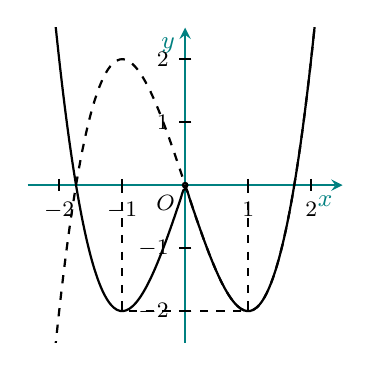
\begin{tikzpicture}[thick,>=stealth,scale=0.8] 
	\clip(-2.5,-2.5) rectangle (2.5,2.5);
	\draw[->,teal] (-2.5,0) -- (2.5,0) node[below left] {\small $x$};
	\draw[->,teal] (0,-2.5) -- (0,2.5) node[below left] {\small $y$};
	\foreach \x in {-2,-1,1,2}\draw (\x,0.1)--(\x,-0.1) node [below] {\footnotesize $\x$};
	\foreach \y in {-2,-1,1,2}\draw (0.1,\y)--(-0.1,\y) node [left] {\footnotesize $\y$};
	\draw [fill=white,draw=black] (0,0) circle (1pt)node[below left] {\footnotesize $O$};
	\draw[thick,black,dashed,smooth,samples=100,domain=-2.5:2.5] plot(\x,{(\x)^3-3*(\x)});
	\draw[thick,black,smooth,samples=100,domain=-2.5:2.5] plot(\x,{abs((\x))^3-3*abs((\x))});
	\draw[dashed] (1,0)--(1,-2)--(0,-2);
	\draw[dashed] (-1,0)--(-1,-2)--(0,-2);
	\end{tikzpicture}
}
\loigiai{
	Ta có: $3$ hàm số của các phương án $y=\left|x^3+3x\right|$, $y=|x|^3+3|x|$,  $y=\left|x^3-3x\right|$ đều là các hàm số có giá trị không âm $\forall x\in \mathbb{R}$. Vậy phương án $y=|x|^3-3|x|$ đúng.
}
\end{ex}
\begin{ex}%[2D1K5-1]%Câu 12.
\immini{
	Hàm số $y=ax^3+bx^2+cx+d$ có đồ thị như hình vẽ sau (đồ thị không đi qua gốc tọa độ). Mệnh đề nào sau đây \textbf{đúng}?
	\choice
	{$a<0;b<0;c<0;d>0$}
	{$a<0;b>0;c<0;d>0$}
	{\True $a<0;b>0;c>0;d>0$}
	{$a<0;b<0;c>0;d>0$}
}{
	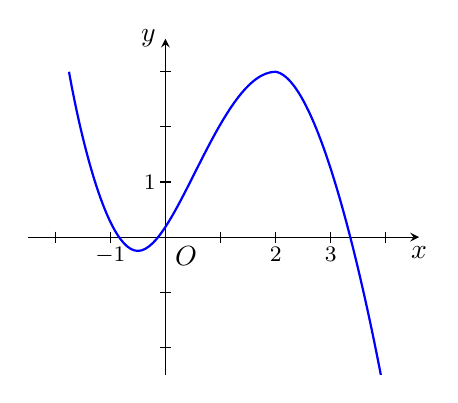
\begin{tikzpicture}[>=stealth,scale=0.7]
	\clip(-2.5,-2.5) rectangle (4.8,3.8);
	\draw[->] (-2.5,0)--(4.6,0) node[below] {$x$};
	\draw[->] (0,-2.5)--(0,3.6) node[left] {$y$};
	\foreach \x in {-2,-1,1,2,3,4}\draw (\x,0.1)--(\x,-0.1) ;
	\foreach \y in {-2,-1,1,2,3}\draw (0.1,\y)--(-0.1,\y) ;
	\coordinate (A) at (-1.75,3.0);
	\coordinate (B) at (-0.5,-0.25);
	\coordinate (C) at (2.0,3.0);
	\coordinate (D) at (4,-3);
	\draw (0,0) node [below right] {$O$};
	\draw[blue,thick] 
	(A) .. controls +(-80:0.0) and +(180:0.7) ..
	(B) .. controls +(0:0.7) and +(-180:1.0) ..
	(C) .. controls +(-10:1.0) and +(120:0.0) ..
	(D);
	\draw (0,1) node[left]{\footnotesize $1$};
	\draw (-1,0) node[below]{\footnotesize $-1$};
	\draw (2,0) node[below]{\footnotesize $2$};
	\draw (3,0) node[below]{\footnotesize $3$};
	% \draw (1,0) node[below left]{\footnotesize $1$};
	\end{tikzpicture}
}
\loigiai{
	Gọi $x_1;x_2$ là hoành độ hai điểm cựu trị của đồ thị hàm số thì $x_1;x_2$ là nghiệm của phương trình $y'=3ax^2+2bx+c=0$.\\
	Dựa vào đồ thị ta có: $\heva{&x_1+x_2=-\dfrac{b}{3a}>0\\&x_1x_2=\dfrac{c}{3a}<0}$ vì $a<0$ nên $b>0; c>0$.}
\end{ex}

\begin{ex}%[2D1Y5-1]%Câu 13.
\immini{
	Giá trị $a, b$ để hàm số $y=\dfrac{ax+b}{x-1}$ có đồ thị như hình bên là
	\choice
	{$a=-1,b=2$}
	{$a=-1,b=-2$}
	{\True $a=1,b=2$}
	{$a=-1,b=-2$}
}{
	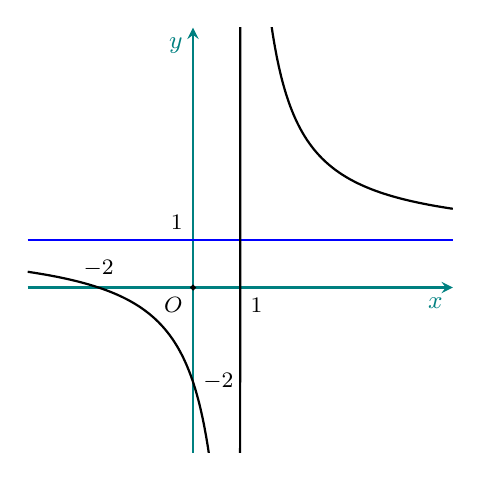
\begin{tikzpicture}[thick,>=stealth,scale=0.6] 
	\clip(-3.5,-3.5) rectangle (5.5,5.5);
	\draw[->,teal] (-3.5,0) -- (5.5,0) node[below left] {\small $x$};
	\draw[->,teal] (0,-3.5) -- (0,5.5) node[below left] {\small $y$};
	\draw[blue] (-3.5,1.0) -- (5.5,1.0);
	\draw [fill=white,draw=black] (0,0) circle (1pt)node[below left] {\footnotesize $O$};
	\draw(1.0,0) node[below right] {\footnotesize $1$};
	\draw (-2,0) node[above] {\footnotesize $-2$};
	\draw (0,-2) node[right] {\footnotesize $-2$};
	\draw (0,1.0) node[above left] {\footnotesize $1$};
	\draw[thick,black,smooth,samples=100,domain=-3.5:5.5] plot(\x,{(\x+2)/(\x-1)});
	\end{tikzpicture}
}
\loigiai{
	Ta có đồ thị hàm số $y=\dfrac{ax+b}{x-1}$ có tiệm cận ngang $y=a\Rightarrow a=1$, đồ thị hàm số cắt trục tung tại điểm có tọa độ $(0;-b)\Rightarrow b=2$.}
\end{ex}
\begin{ex}%[2D1Y5-1]%Câu 14.
Bảng biến thiên dưới đây là của hàm số nào?
\begin{center}
	
\begin{tikzpicture}
	\tkzTabInit[lgt=1.0,espcl=2.0,deltacl=.5,nocadre]
	{$x$ /.7, $y’$ /.7,$y$ /2}
	{$-\infty$ , $-1$,$0$ , $1$ , $+\infty$}
	\tkzTabLine{,-,0,+,0,-,0,+,}
	\tkzTabVar{+/$+\infty$ ,-/$-4$  ,+/$-3$, -/$-4$,+/$+\infty$}
	\end{tikzpicture}
\end{center}
\choice
{$y=x^4+2x^2-3$}
{$y=-x^4-2x^2-3$}
{\True $y=x^4-2x^2-3$}
{$y=x^4+2x^2+3$}
\loigiai{
	Qua bảng biến thiên ta thấy hàm số trùng phương có $a>0\Rightarrow$ loại đáp án $y=-x^4-2x^2-3$.\\
	Từ bảng biến thiên có điểm cực trị tọa độ $(0;-3)$ thuộc đồ thị nên loại $y=x^4+2x^2+3$.\\
	Từ bảng biến thiên ta thấy có ba cực trị nên $b<0$ loại $y=x^4+2x^2-3$.\\
	Vậy $y=x^4-2x^2-3$ là phương án đúng.
}
\end{ex}
\begin{ex}%[2D1K5-1]%Câu 15.
\immini{
	Hình vẽ bên dưới là một phần đồ thị của hàm số nào?
	\choice
	{\True $y=\dfrac{x-1}{|x|+1}$}
	{$y=\dfrac{x-1}{|x+1|}$}
	{$y=\dfrac{x}{|x|+1}$}
	{$y=\dfrac{-x-1}{|x|+1}$}
}{
	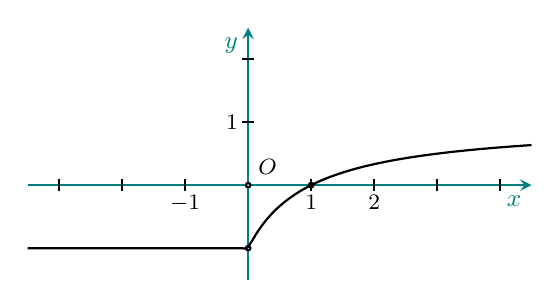
\begin{tikzpicture}[thick,>=stealth,scale=0.8] 
	\clip(-3.5,-1.5) rectangle (4.5,2.5);
	\draw[->,teal] (-3.5,0) -- (4.5,0) node[below left] {\small $x$};
	\draw[->,teal] (0,-1.5) -- (0,2.5) node[below left] {\small $y$};
	\foreach \x in {-3,-2,-1,1,2,3,4}\draw (\x,0.1)--(\x,-0.1) ;
	\foreach \y in {1,2}\draw (0.1,\y)--(-0.1,\y) ;
	\draw [fill=white,draw=black] (0,0) circle (1pt)node[above right] {\footnotesize $O$};
	\draw(-1.0,0) node[below] {\footnotesize $-1$};
	\draw (1,0) node[below] {\footnotesize $1$};
	\draw (2,0) node[below] {\footnotesize $2$};
	\draw (0,1.0) node[left] {\footnotesize $1$};
	\draw [fill=white,draw=black] (1,0) circle (1pt);
	\draw [fill=white,draw=black] (0,-1) circle (1pt);
	\draw[thick,black,smooth,samples=100,domain=-3.5:4.5] plot(\x,{(\x-1)/(abs(\x)+1)});
	\end{tikzpicture}
}
\loigiai{
	Ta có: $y=\dfrac{x-1}{|x|+1}=\heva{&\dfrac{x-1}{x+1} \,\,\text{khi}\,\, x\geq 0\\&-1 \,\,\text{khi}\,\, x<0}$ nên đồ thị gồm hai phần:\\
	Phần 1: Là đồ thị hàm số $y=\dfrac{x-1}{x+1}$ phần bên phải trục tung.\\
	Phần 2: Là đồ thị hàm số $y=-1$ phần bên trái trục tung.}
\end{ex}
\begin{ex}%[2D1K5-1]%Câu 16.
\immini{
	Cho hàm số bậc ba $y=ax^3+bx^2+cx+d$ có đồ thị như nhình vẽ. Giá trị nhỏ nhất của biểu thức $P=a^2+c^2+b+1$ là
	\choice
	{$\dfrac{1}{5}$}
	{$1$}
	{\True $\dfrac{5}{8}$}
	{$\dfrac{1}{3}$}
}{
	\begin{tikzpicture}[thick,>=stealth,scale=1.0] 
	\clip(-1.5,-2.5) rectangle (3.5,3.0);
	\draw[->,teal] (-1.5,0) -- (3.5,0) node[below left] {\small $x$};
	\draw[->,teal] (0,-2.5) -- (0,3.0) node[below left] {\small $y$};
	\foreach \x in {-1,1,2,3}\draw (\x,0.1)--(\x,-0.1);
	\foreach \y in {-2,-1,1,2}\draw (0.1,\y)--(-0.1,\y);
	\draw [fill=white,draw=black] (0,0) circle (1pt)node[below left] {\footnotesize $O$};
	\draw[thick,black,smooth,samples=100,domain=-2.5:2.5] plot(\x,{(\x)^3-3*(\x)^2+3*(\x)});
	\draw (0,-2) node[left] {\footnotesize $-2$};
	\draw (0,2) node[left] {\footnotesize $2$};
	\end{tikzpicture}
}
\loigiai{
	$y^/=3ax^2+2bx+c$ có $\Delta^/=b^2-3ac$.\\
	Dựa vào đồ thị, ta có $y^/=0$ có nghiệm kép (bội 2)\\
	$ \Leftrightarrow\heva{&a\neq 0\\&{\Delta}^/=0}\Leftrightarrow\heva{&a\neq 0\\&b^2=3ac\geq 0.} $ \\
	Vậy	$P=a^2+c^2+b+1\geq 2ac+b+1=\dfrac{2}{3}b^2+b+1\geq\dfrac{5}{8}$.}
\end{ex}

\begin{ex}%[2D1G5-1]%Câu 17.
\immini{
	Cho hàm số $y=ax^3+bx^2+cx+d$ có đồ thị như hình vẽ. Tính $S=a+b$?
	\choice
	{$S=0$}
	{$S=1$}
	{$S=-1$}
	{\True $S=-2$}
}{
	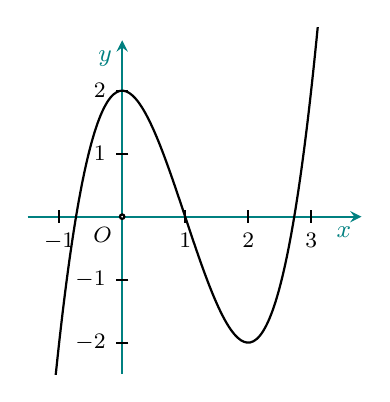
\begin{tikzpicture}[thick,>=stealth,scale=0.8] 
	\clip(-1.5,-2.5) rectangle (3.8,3.0);
	\draw[->,teal] (-1.5,0) -- (3.8,0) node[below left] {\small $x$};
	\draw[->,teal] (0,-2.5) -- (0,2.8) node[below left] {\small $y$};
	\foreach \x in {-1,1,2,3}\draw (\x,0.1)--(\x,-0.1)node [below] {\footnotesize $\x$} ;
	\foreach \y in {-2,-1,1,2}\draw (0.1,\y)--(-0.1,\y)node [left] {\footnotesize $\y$};
	\draw [fill=white,draw=black] (0,0) circle (1pt)node[below left] {\footnotesize $O$};
	\draw[thick,black,smooth,samples=100,domain=-1.5:3.5] plot(\x,{(\x)^3-3*(\x)^2+2});
	%\draw (0,-2) node[left] {\footnotesize $-2$};
	%\draw (0,2) node[left] {\footnotesize $2$};
	\end{tikzpicture}
}
\loigiai{
	Vì đồ thị hàm số cắt trục tung tại điểm $y=2$ nên $d=2$.\\
	Ta có: $y'=3ax^2+2bx+c$.\\
	Hàm số đạt cực trị tại $x=0$ và $x=2$ nên
	\[\heva{&y'(0)=0\\&y'(2)=0}\Leftrightarrow\heva{&c=0\\&12a+4b+c=0}\Leftrightarrow\heva{&c=0\\&b=-3a \quad (1).}\] 
	Từ đồ thị ta nhận thấy $y(2)=-2\Leftrightarrow 8a+4b+d=-2\Leftrightarrow 8a+4b=-4\Leftrightarrow 2a+b=-1 \quad (2)$.\\
	Thay $(1)$ vào $(2)$ ta tìm được $a=1,b=-3$.\\
	Vậy $S=-2$.}
\end{ex}

\begin{ex}%[2D1K5-1]%Câu 18.
\immini{
	Đồ thị hàm số $y=ax^3+bx^2+c$ cho như hình bên. Mệnh đề nào sau đây là \textbf{đúng}?
	\choice
	{$a<0,b>0,c>0$}
	{\True $a<0,b>0,c<0$}
	{$a>0,b>0,c>0$}
	{$a>0,b>0,c<0$}
}{
	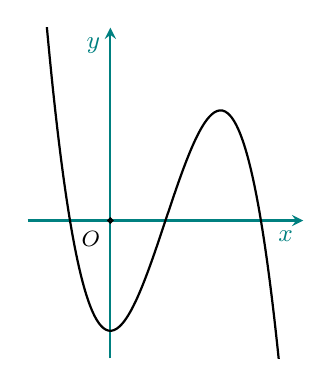
\begin{tikzpicture}[thick,>=stealth,scale=0.7] 
	\clip(-1.5,-2.5) rectangle (3.5,3.5);
	\draw[->,teal] (-1.5,0) -- (3.5,0) node[below left] {\small $x$};
	\draw[->,teal] (0,-2.5) -- (0,3.5) node[below left] {\small $y$};
	%\foreach \x in {-1,1,2,3}\draw (\x,0.1)--(\x,-0.1)node [below] {\footnotesize $\x$} ;
	%\foreach \y in {-2,-1,1,2,3}\draw (0.1,\y)--(-0.1,\y)node [left] {\footnotesize $\y$};
	\draw [fill=white,draw=black] (0,0) circle (1pt)node[below left] {\footnotesize $O$};
	\draw[thick,black,smooth,samples=100,domain=-1.5:3.5] plot(\x,{-(\x)^3+3*(\x)^2-2});
	%\draw (0,-2) node[left] {\footnotesize $-2$};
	%\draw (0,2) node[left] {\footnotesize $2$};
	\end{tikzpicture}
}
\loigiai{
	Quan sát đồ thị ta thấy.\\
	+ Đồ thị hàm số cắt $Oy$ tại điểm có tung độ là $c$ suy ra $c<0$. Loại $a<0,b>0,c>0$, $a>0,b>0,c>0$.\\
	+ Khi $x\to+\infty$ thì $y\to-\infty$ suy ra $a<0$. Loại $a>0,b>0,c<0$.\\
	Vậy $a<0,b>0,c<0$ là đáp án đúng.}
\end{ex}
\begin{ex}%[2D1G5-1]%Câu 19.
\immini{
	Cho hàm số $y=-2x^3+bx^2+cx+d$ có đồ thị như hình dưới. Khẳng định nào sau đây \textbf{đúng}?
	\choice
	{$bcd=-144$}
	{$c^2<b^2+d^2$}
	{\True $b+c+d=1$}
	{$b+d<c$}
}{
	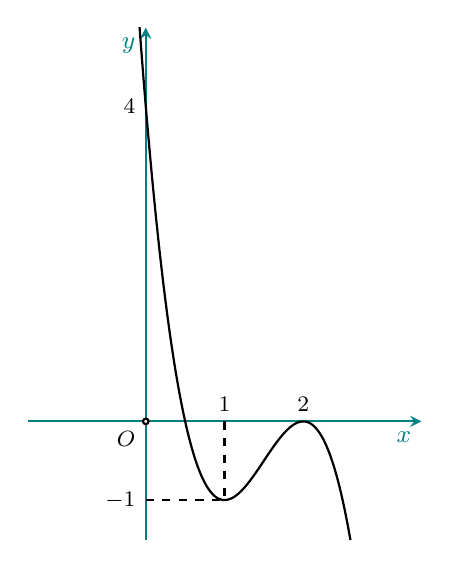
\begin{tikzpicture}[thick,>=stealth,scale=1.0] 
	\clip(-1.5,-1.5) rectangle (3.5,5.0);
	\draw[->,teal] (-1.5,0) -- (3.5,0) node[below left] {\small $x$};
	\draw[->,teal] (0,-2.5) -- (0,5.0) node[below left] {\small $y$};
	%\foreach \x in {-1,1,2,3}\draw (\x,0.1)--(\x,-0.1)node [below] {\footnotesize $\x$} ;
	%\foreach \y in {-2,-1,1,2,3}\draw (0.1,\y)--(-0.1,\y)node [left] {\footnotesize $\y$};
	\draw [fill=white,draw=black] (0,0) circle (1pt)node[below left] {\footnotesize $O$};
	\draw[thick,black,smooth,samples=100,domain=-1.5:3.5] plot(\x,{-2*(\x)^3+9*(\x)^2-12*(\x)+4});
	\draw (1,0) node[above] {\footnotesize $1$};
	\draw (2,0) node[above] {\footnotesize $2$};
	\draw (0,4) node[left] {\footnotesize $4$};
	\draw (0,-1) node[left] {\footnotesize $-1$};
	\draw[dashed] (1,0)--(1,-1)--(0,-1);
	\end{tikzpicture}
}
\loigiai{
	Từ đồ thị ta có $x=0 \Rightarrow y(0) =0 \Leftrightarrow d=4$.\\
	Mặt khác, $y'= -6x^2+2bx+c$.\\
	Từ đồ thị suy ra $y'=0$ có hai nghiệm giả sử $x_1=1;x_2=2$.\\
	Do đó theo Vi-et ta có: 
	\[\heva{  
		& x_1+x_2=-\dfrac{2b}{-6}\\
		& x_1\cdot x_2=\dfrac{c}{-6}
	} \Rightarrow
	\heva{  
		& -\dfrac{2b}{-6}=3\\
		& \dfrac{c}{-6}=2
	} \Leftrightarrow
	\heva{  
		& b=9\\
		& c=-12
	}
	\]
	Do đó $a\cdot b\cdot c=-432; b+c+d=-1; b+d>c; b^2+d^2>c^2$.\\
	Vậy $b^2+d^2>c^2$ là đúng?
}
\end{ex}

\begin{ex}%[2D1G5-1]%Câu 20.
Cho hàm số $y=f(x) = (x-1)(x^2-2x-3)$ có đồ thị như hình vẽ. 
\begin{center}
	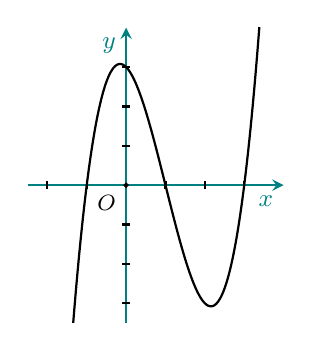
\begin{tikzpicture}[thick,>=stealth,scale=0.5] 
	\clip(-2.5,-3.5) rectangle (4.0,4.0);
	\draw[->,teal] (-2.5,0) -- (4.0,0) node[below left] {\small $x$};
	\draw[->,teal] (0,-3.5) -- (0,4.0) node[below left] {\small $y$};
	\foreach \x in {-3,-2,-1,1,2,3}\draw (\x,0.1)--(\x,-0.1);
	\foreach \y in {-3,-2,-1,1,2,3}\draw (0.1,\y)--(-0.1,\y);
	\draw [fill=white,draw=black] (0,0) circle (1pt)node[below left] {\footnotesize $O$};
	\draw[thick,black,smooth,samples=100,domain=-1.5:3.5] plot(\x,{((\x)-1)*((\x)^2-2*(\x)-3)});
	%\draw (0,-2) node[left] {\footnotesize $-2$};
	%\draw (0,2) node[left] {\footnotesize $2$};
	\end{tikzpicture}
\end{center}
Hình vẽ dưới đây là đồ thị của hàm số nào?
\begin{center}
	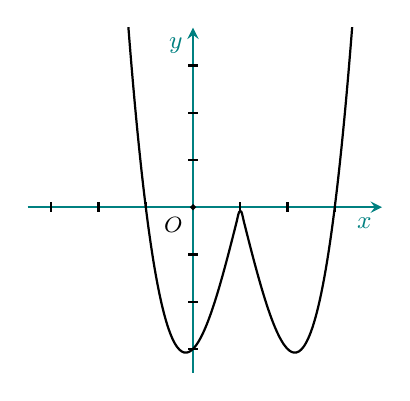
\begin{tikzpicture}[thick,>=stealth,scale=0.6] 
	\clip(-3.5,-3.5) rectangle (4.0,3.8);
	\draw[->,teal] (-3.5,0) -- (4.0,0) node[below left] {\small $x$};
	\draw[->,teal] (0,-3.5) -- (0,3.8) node[below left] {\small $y$};
	\foreach \x in {-3,-2,-1,1,2,3}\draw (\x,0.1)--(\x,-0.1);
	\foreach \y in {-3,-2,-1,1,2,3}\draw (0.1,\y)--(-0.1,\y);
	\draw [fill=white,draw=black] (0,0) circle (1pt)node[below left] {\footnotesize $O$};
	\draw[thick,black,smooth,samples=100,domain=-1.5:3.5] plot(\x,{abs((\x)-1)*((\x)^2-2*(\x)-3)});
	%\draw (0,-2) node[left] {\footnotesize $-2$};
	%\draw (0,2) node[left] {\footnotesize $2$};
	\end{tikzpicture}
\end{center}
\choice
{$y=|(x-1)(x^2-2x-3)|$}
{$y=(x-1)|x^2-2x-3|$}
{\True $y=|x-1|(x^2-2x-3)$}
{$y=(|x|-1)(x^2-2|x|-3)$}
\loigiai{
	\immini{
		Ta có: $y=(x-1)(x^2-2x-3)$.\\
		Khi đó $y_1=|x-1|(x^2-2x-3) = 
		\begin{cases}
		y \, \text{ nếu } \, x-1\geq 0 \hspace{0.5cm} (1)\\
		-y \, \text{ nếu } \, x -1< 0. \hspace{0.5cm} (2)
		\end{cases}	
		$\\
		Do đó đồ thị hàm số $(C_1)$ được suy ra từ đồ thị hàm số $(C)$ như sau:\\
		- Giữ nguyên phần đồ thị của $(C)$ nằm trên miền $x-1>0$ (do $(1)$).\\
		- Lấy đối xứng qua trục hoành phần đồ thị $(C)$ nằm trên miền $x-1<0$ (do $(2)$).
	}{
		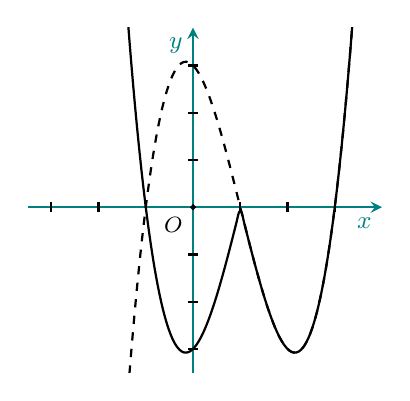
\begin{tikzpicture}[thick,>=stealth,scale=0.6] 
		\clip(-3.5,-3.5) rectangle (4.0,3.8);
		\draw[->,teal] (-3.5,0) -- (4.0,0) node[below left] {\small $x$};
		\draw[->,teal] (0,-3.5) -- (0,3.8) node[below left] {\small $y$};
		\foreach \x in {-3,-2,-1,1,2,3}\draw (\x,0.1)--(\x,-0.1);
		\foreach \y in {-3,-2,-1,1,2,3}\draw (0.1,\y)--(-0.1,\y);
		\draw [fill=white,draw=black] (0,0) circle (1pt)node[below left] {\footnotesize $O$};
		\draw[thick,dashed,black,smooth,samples=100,domain=-1.5:3.5] plot(\x,{((\x)-1)*((\x)^2-2*(\x)-3)});
		\draw[thick,black,smooth,samples=100,domain=-1.5:3.5] plot(\x,{abs((\x)-1)*((\x)^2-2*(\x)-3)});
		%\draw (0,-2) node[left] {\footnotesize $-2$};
		%\draw (0,2) node[left] {\footnotesize $2$};
		\end{tikzpicture}
	}
}
\end{ex}

\begin{ex}%[2D1G5-1]%Câu 21.
Cho hàm số bậc bốn $f(x)=ax^4+bx^3+cx^2+\mathrm{\,d}x+e$, $a\neq 0$. Biết rằng các hệ số $a,b,c,d,e$ là các số nguyên không âm và không lớn hơn $8$ và $f(9)=32078$. Tính tổng các hệ số $S=a+b+c+d+e$. 
\choice
{$S=4$}
{$S=10$}
{$S=12$}
{\True $S=14$}
\loigiai{
	Ta có các hệ số $a,b,c,d,e$ là các số nguyên không âm và không lớn hơn 8, suy ra các hệ số không chia hết cho $9$. Vì vậy do $f(9)=32078$ nên $e$ chính là số dư khi chia $32078$ cho 9 $\Rightarrow e=2$.\\
	+) $f(9)-2=\left(a\cdot 9^3+b\cdot 9^2+c\cdot 9+d\right)9$ nên $d$ chính là số dư của $\dfrac{f(9)-2}{9}$ khi chia cho $9$ nên $d=0$ (do 32076 chia hết cho $9^2$).\\
	+) $f(9)-2=\left(a\cdot 9^2+b\cdot 9+c\right)9^2$ nên $c$ chính là số dư của $\dfrac{f(9)-2}{9^2}$ khi chia cho 9 nên $c=0$ (do 32076 chia hết cho $9^3$).\\
	+) $f(9)-2=(a\cdot 9+b)9^3$ nên $b$ chính là số dư của $\dfrac{f(9)-2}{9^3}$ khi chia cho 9 nên $b=8$.\\
	+) $f(9)-2=(a\cdot 9+8)9^3$ nên $a=4$.\\
	Vậy $S=14$.}
\end{ex}
\Closesolutionfile{ans}